\documentclass[11pt,a4paper]{article}
\usepackage{nabiadoc}
\usepackage{tikz}
\usetikzlibrary{positioning,arrows.meta,fit,calc}
\usepackage{caption}
\captionsetup[lstlisting]{justification=raggedright, singlelinecheck=false, font=small, labelfont=bf}
\usepackage{tabularx}

% Generated at build time by extract_snippets.py: excerpt locations, the MCP
% tool catalogue (tools.tex) and the AI configuration fields (config.tex).
\input{snippets.tex}
\newcommand{\snippetsource}[1]{\csname snippet@#1\endcsname}
\newcommand{\snippet}[3]{%
  \lstinputlisting[language=#2, caption={#3\\{\footnotesize\ttfamily\snippetsource{#1}}}]{#1.txt}}
% A prompt: plain text, wrapped.
\newcommand{\prompt}[2]{%
  \lstinputlisting[language={}, basicstyle=\ttfamily\scriptsize, keywordstyle={}, commentstyle={},
                   caption={#2\\{\footnotesize\ttfamily\snippetsource{#1}}}]{#1.txt}}
\lstset{basicstyle=\ttfamily\scriptsize, captionpos=t, numbers=none, aboveskip=8pt, belowskip=8pt,
        tabsize=4, keepspaces=true, breaklines=true, postbreak=\mbox{\textcolor{gray}{$\hookrightarrow$}\space}}
\renewcommand{\lstlistingname}{Code}

% Pointers from a concept to its code.
\newcommand{\coderef}[1]{{\footnotesize\texttt{\snippetsource{#1}}}}
\newenvironment{codepointers}{%
  \par\smallskip\begingroup\footnotesize\noindent\textcolor{blue!50!black}{\textbf{Code}}\par\nopagebreak
  \begin{list}{}{\setlength{\leftmargin}{1.2em}\setlength{\itemsep}{0pt}\setlength{\parsep}{0pt}\setlength{\topsep}{1pt}}}%
  {\end{list}\endgroup\smallskip}
\newcommand{\codeitem}[2]{\item #2 --- \texttt{\snippetsource{#1}}}

% MCP tool catalogue entries (tools.tex).
\newcommand{\toolentry}[3]{\subsubsection*{\texttt{#1}}\vspace{-0.6em}
  \noindent{\footnotesize\textcolor{gray!30!black}{\emph{#2}\hfill\texttt{#3}}}\par\smallskip}
\newcommand{\modelentry}[2]{\subsubsection*{Input schema \texttt{#1}}\vspace{-0.6em}
  \noindent{\footnotesize\textcolor{gray!30!black}{\emph{pydantic model}\hfill\texttt{#2}}}\par\smallskip}
\newenvironment{toolparams}{\begin{description}\footnotesize\setlength{\itemsep}{0pt}\setlength{\parsep}{0pt}}{\end{description}}

\title{nabia: Architecture, Methodology and Reference\\[0.3em]
\large A systematic trend strategy platform: C++ numerical core, Python layer, AI agents and web application}
\author{nabia documentation}
\date{October 2026}

\begin{document}
\maketitle

\begin{abstract}
This document is the reference for the whole nabia project. It describes the architecture,
then every method the project implements, stated mathematically, with proofs where a
property is relied on. It covers:
\begin{itemize}
  \item the C++ numerical core: time series, signal filters, forecasters, five optimizers,
        risk measures, risk budgeting and the walk-forward portfolio engine;
  \item the command-line application, the Python bindings and the market data pipeline;
  \item the AI layer: the three agents with their complete prompts, the MCP servers with
        every tool's description and input schema, the agent loop, the statistics the agents
        see, and how news sentiment and relevance are produced and aggregated;
  \item the web application and the job runner.
\end{itemize}
Each concept points to the code that implements it, by file and line range, and the key
code is shown in excerpts. Excerpts, prompts, tool descriptions and configuration fields
are \emph{extracted from the source when the document is built}, so they are the text the
programs actually use, and a renamed function stops the build instead of leaving a stale
reference.
\end{abstract}

\tableofcontents
\clearpage

%==============================================================================
\part{Overview}

\section{Purpose}

nabia is a platform for researching and running \emph{systematic trend strategies} across
asset classes: equity indices, government bond futures, commodities and crypto. A strategy
has four stages, and the project provides a component for each:
\begin{enumerate}
  \item \textbf{Data}: daily prices from public sources into a SQL database, kept up to
        date incrementally (\S\ref{sec:marketdata}).
  \item \textbf{Signals and views}:
        \begin{itemize}
          \item filters and forecasters that extract trends from noisy prices
                (\S\ref{sec:signal}, \S\ref{sec:forecast});
          \item statistical and news analysis on top of these, done by AI agents
                (\S\ref{sec:agents}--\ref{sec:sentiment}).
        \end{itemize}
  \item \textbf{Allocation}: \emph{risk budgeting} decides each asset's share of portfolio
        risk. A deterministic engine turns budgets into weights, scales them to a volatility
        target and simulates trading with costs (\S\ref{sec:riskbudgeting}, \S\ref{sec:engine}).
  \item \textbf{Evaluation and operation}: walk-forward backtests without look-ahead,
        performance metrics, and a web application to run jobs and audit every decision
        (\S\ref{sec:metrics}, \S\ref{sec:web}).
\end{enumerate}

The central design decision is to separate \emph{who decides the risk budgets} from
\emph{how budgets become positions}:
\begin{itemize}
  \item Budgets are decided by a fixed rule, by equal risk, or by AI agents.
  \item Positions come from a tested numerical engine.
\end{itemize}
Agents never set weights. They choose budgets within bounds, and the engine computes the
weights, so an agent's influence is bounded and every decision is reproducible from its
stored budgets.

\section{Architecture}\label{sec:architecture}

\begin{figure}[ht]
\centering
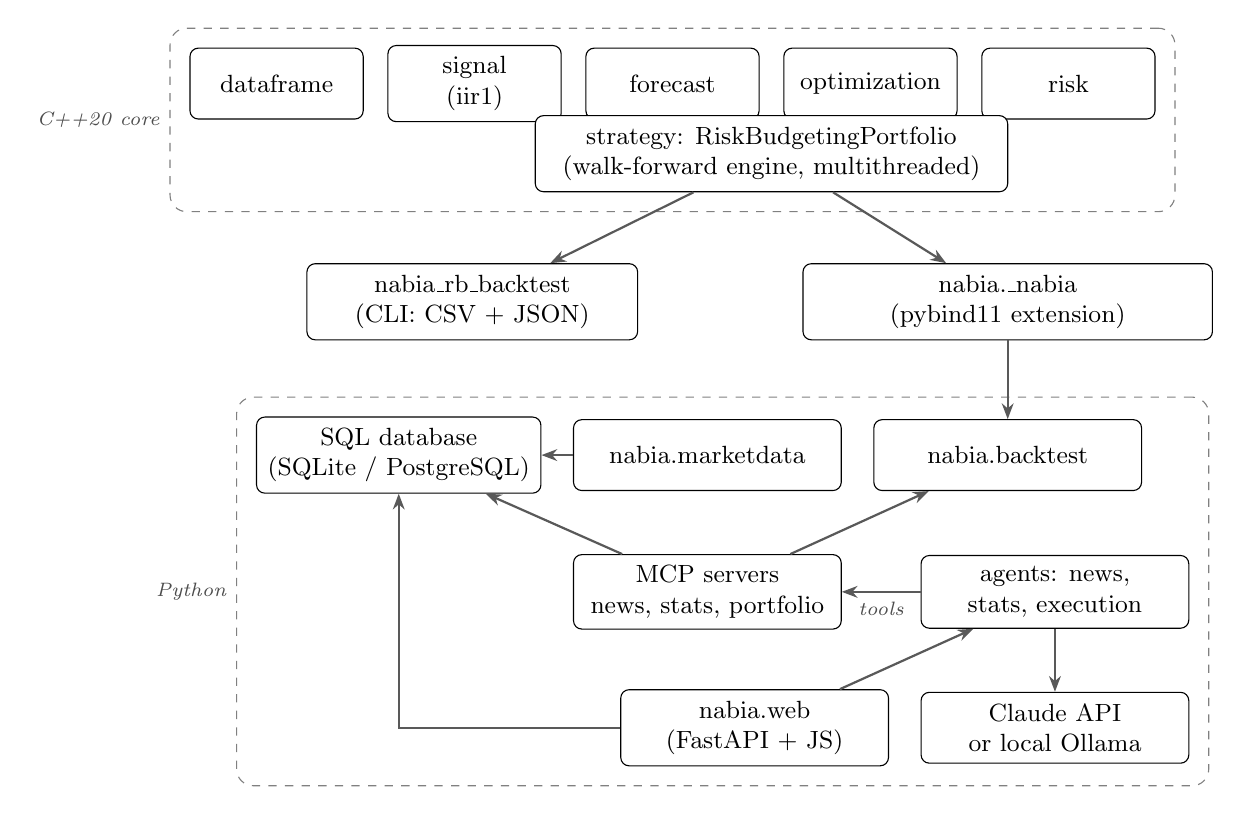
\begin{tikzpicture}[
  box/.style={draw, rounded corners=3pt, align=center, minimum height=9mm, font=\small, fill=white, inner sep=4pt},
  layer/.style={draw, dashed, rounded corners=6pt, inner sep=7pt, gray},
  arrow/.style={-{Stealth[length=2mm]}, thick, gray!70!black},
  lbl/.style={font=\scriptsize\itshape, gray!60!black}]
  \node[box, minimum width=22mm] (df) {dataframe};
  \node[box, right=3mm of df, minimum width=22mm] (sig) {signal\\(iir1)};
  \node[box, right=3mm of sig, minimum width=22mm] (fc) {forecast};
  \node[box, right=3mm of fc, minimum width=22mm] (opt) {optimization};
  \node[box, right=3mm of opt, minimum width=22mm] (risk) {risk};
  \node[box, below=4mm of $(fc)!0.5!(opt)$, minimum width=60mm] (strat) {strategy: RiskBudgetingPortfolio\\(walk-forward engine, multithreaded)};
  \node[layer, fit=(df)(risk)(strat), label={[lbl]left:C++20 core}] (core) {};
  \node[box, below=9mm of strat, xshift=-38mm, minimum width=42mm] (cli) {nabia\_rb\_backtest\\(CLI: CSV + JSON)};
  \node[box, below=9mm of strat, xshift=30mm, minimum width=52mm] (bind) {nabia.\_nabia\\(pybind11 extension)};
  \node[box, below=10mm of bind, minimum width=34mm] (pf) {nabia.backtest};
  \node[box, left=4mm of pf, minimum width=34mm] (md) {nabia.marketdata};
  \node[box, left=4mm of md, minimum width=30mm] (db) {SQL database\\(SQLite / PostgreSQL)};
  \node[box, below=8mm of md, minimum width=34mm] (mcp) {MCP servers\\news, stats, portfolio};
  \node[box, right=10mm of mcp, minimum width=34mm] (agents) {agents: news,\\stats, execution};
  \node[box, below=8mm of agents, minimum width=34mm] (llm) {Claude API\\or local Ollama};
  \node[box, left=4mm of llm, minimum width=34mm] (web) {nabia.web\\(FastAPI + JS)};
  \node[layer, fit=(db)(pf)(mcp)(agents)(llm)(web), label={[lbl]left:Python}] (py) {};
  \draw[arrow] (strat) -- (cli);
  \draw[arrow] (strat) -- (bind);
  \draw[arrow] (bind) -- (pf);
  \draw[arrow] (md) -- (db);
  \draw[arrow] (mcp) -- (db);
  \draw[arrow] (mcp) -- (pf);
  \draw[arrow] (agents) -- node[lbl, below]{tools} (mcp);
  \draw[arrow] (agents) -- (llm);
  \draw[arrow] (web) -- (agents);
  \draw[arrow] (web.west) -| (db.south);
\end{tikzpicture}
\caption{Components and dependencies. Arrows point from a component to what it uses.}
\label{fig:architecture}
\end{figure}

\subsection{Layers}
\begin{description}
  \item[C++ core] (\code{include/nabia}, \code{src}): the static library \code{nabia::nabia},
        built with CMake. It uses C++20, Eigen for linear algebra and iir1 for filter
        design. Each module exposes an abstract interface whose parameter struct is owned
        through \code{std::unique\_ptr}:
        \begin{itemize}
          \item \code{IFilter<P>} (\coderef{ifilter});
          \item \code{IForecaster<P>} (\coderef{iforecaster});
          \item \code{IOptimizer<P,R>} (\coderef{ioptimizer});
          \item \code{IRiskMeasure} (\coderef{irisk}).
        \end{itemize}
  \item[Application] \code{nabia\_rb\_backtest} (\code{apps/rb\_backtest}): a backtest from a
        prices CSV and a JSON configuration, written to CSV.
  \item[Python bindings] (\code{python/src}): the pybind11 module \code{nabia.\_nabia}
        exposes the engine, and the \code{nabia} package wraps it in pandas objects.
  \item[Python packages]
        \begin{itemize}
          \item \code{nabia.marketdata}: download and storage;
          \item \code{nabia.ai}: agents, MCP servers and pipeline;
          \item \code{nabia.web}: web application and job runner.
        \end{itemize}
  \item[Storage] one SQL database holds prices, news, statistics reports, decisions, agent
        transcripts, jobs, job logs and backtest runs. Access goes through SQLAlchemy Core
        with portable types, so moving from SQLite to PostgreSQL changes only the URL.
\end{description}

\subsection{Directory map}
\begin{center}\small
\begin{tabular}{@{}l>{\raggedright\arraybackslash}p{10cm}@{}}
\toprule
Path & Contents \\
\midrule
\code{include/nabia/dataframe} & \code{TimeSeries}, \code{DataFrame}, the \code{TimeIndex} concept \\
\code{include/nabia/signal} & \code{IFilter}, \code{EWMA}, \code{ButterworthBandPass}, smoothing helpers \\
\code{include/nabia/forecast} & \code{IForecaster}, SES, Kalman filter, Gaussian process, kernels \\
\code{include/nabia/optimization} & \code{IOptimizer}; \code{convex/}: constraints, L-BFGS, augmented Lagrangian, SQP; \code{nongradopt/}: Nelder--Mead, differential evolution \\
\code{include/nabia/risk} & \code{IRiskMeasure}, volatility, VaR, ES, \code{RiskBudgeting<Measure>} \\
\code{include/nabia/stats} & descriptive statistics, normal density, CDF and quantile \\
\code{include/nabia/strategy} & \code{RiskBudgetingPortfolio}, performance metrics \\
\code{apps/rb\_backtest} & command-line backtest (CSV and JSON) \\
\code{python/nabia} & \code{portfolio}, \code{marketdata}, \code{ai} (agents, servers, pipeline), \code{web} \\
\code{doc}, \code{docs} & LaTeX sources (built by CMake) and generated PDFs \\
\code{tests}, \code{python/tests} & Catch2 and pytest suites \\
\bottomrule
\end{tabular}
\end{center}

\subsection{Build}
CMake presets (\code{debug}, \code{release}, \code{asan}, \code{python}) configure the build,
with warnings treated as errors. Dependencies are found on the system or fetched: Eigen,
iir1, Catch2, nlohmann/json and pybind11. The documents are built by the \code{nabia\_docs}
target. For this document it first runs \code{doc/project/extract\_snippets.py}, which
writes the excerpts, the code locations, the tool catalogue of \S\ref{sec:tools} and the
configuration table of \S\ref{sec:aiconfig}.

%==============================================================================
\part{The numerical core (C++)}

\section{Time series containers}\label{sec:dataframe}

All numerical code works on Eigen matrices, but financial data is indexed by time.
\code{TimeSeries<Index>} and \code{DataFrame<Index>} pair an Eigen vector or matrix (rows
are times) with a \emph{strictly increasing} index:
\begin{itemize}
  \item The index type satisfies the \code{TimeIndex} concept (copyable and totally
        ordered): calendar dates, timestamps or integers.
  \item Construction validates the shapes, the ordering and unique column names.
  \item Time lookups use binary search.
\end{itemize}

\paragraph{Alignment.} Markets have different holidays. A cross-asset backtest keeps only
the dates where every asset has a finite price.

\paragraph{Returns.} Simple returns $r_t=P_t/P_{t-1}-1$ (\code{pct\_change}) or log returns
$\log(P_t/P_{t-1})$ are computed between consecutive \emph{kept} rows. A return can
therefore span a removed holiday. That is the right convention for a portfolio that can
only trade when all its markets are open.

\snippet{df_drop_missing}{C++}{Alignment: keep rows where every column is finite}
\begin{codepointers}
  \codeitem{time_index}{\code{TimeIndex} concept}
  \codeitem{timeseries}{\code{TimeSeries}}
  \codeitem{dataframe}{\code{DataFrame}}
  \codeitem{pct_change}{simple returns}
  \codeitem{log_returns}{log returns}
\end{codepointers}

\section{Signal extraction}\label{sec:signal}

Filters implement \code{IFilter<P>}. They are \emph{causal}: output $t$ uses inputs up to
$t$ only. Two modes are supported:
\begin{itemize}
  \item streaming: \code{process(x)}, one sample at a time, keeping state;
  \item batch: \code{apply(signal)}, from a fresh state, without disturbing the streaming
        state.
\end{itemize}
Filter design is delegated to iir1, behind a private implementation struct (pimpl), so iir1
never appears in public headers.

\subsection{Exponentially weighted moving average}
The EWMA is the one-pole low-pass
\[
  y_t=\alpha x_t+(1-\alpha)y_{t-1},\qquad H(z)=\frac{\alpha}{1-(1-\alpha)z^{-1}},\qquad \alpha\in(0,1].
\]
Its DC gain is $H(1)=1$, so a constant input passes unchanged.

\begin{proposition}[Seeding]
Let $\tilde y$ be the EWMA of $x_t-x_0$ started from a zero state. Then $y_t=x_0+\tilde y_t$
equals the recursion started at $y_{-1}=x_0$:
\[
  y_t=\alpha\sum_{k=0}^{t}(1-\alpha)^k x_{t-k}+(1-\alpha)^{t+1}x_0 .
\]
\end{proposition}
\begin{proof}
Unrolling the recursion from $y_{-1}$ gives
$y_t=\alpha\sum_{k=0}^{t}(1-\alpha)^kx_{t-k}+(1-\alpha)^{t+1}y_{-1}$. With a zero state,
$\tilde y_t=\alpha\sum_{k=0}^t(1-\alpha)^k(x_{t-k}-x_0)$. Using
$\alpha\sum_{k=0}^t(1-\alpha)^k=1-(1-\alpha)^{t+1}$, adding $x_0$ gives the formula with
$y_{-1}=x_0$.
\end{proof}
Starting from zero instead would bias the early outputs towards zero, so the filter seeds
with the first sample by default.

\paragraph{Parameterizations.} Two helpers convert the usual parameterizations to $\alpha$:
\begin{itemize}
  \item \code{alpha\_from\_span}$(N)=2/(N+1)$. The mean age of the EWMA weights is
        $\sum_k k\,\alpha(1-\alpha)^k=(1-\alpha)/\alpha$, and that of an $N$-point moving
        average is $(N-1)/2$. Equating the two gives $\alpha=2/(N+1)$.
  \item \code{alpha\_from\_halflife}$(h)=1-2^{-1/h}$. This solves $(1-\alpha)^h=\tfrac12$:
        the weight $h$ steps back is half the newest weight.
\end{itemize}

\snippet{ewma_impl}{C++}{EWMA on iir1's one-pole section, with first-sample seeding}
\begin{codepointers}
  \codeitem{ewma_class}{class and parameters}
  \codeitem{ewma_alphas}{span and half-life conversions}
  \codeitem{moving_average}{simple moving average helper (rolling sum, $O(n)$)}
\end{codepointers}

\subsection{Butterworth band-pass}
A causal Butterworth band-pass isolates trend cycles between two frequencies
$0<f_\ell<f_h<f_s/2$. It is built in three steps.
\begin{enumerate}
  \item \textbf{Analog prototype.} The order-$N$ low-pass prototype is maximally flat:
        \[
          |H(j\Omega)|^2=\frac{1}{1+\Omega^{2N}},
        \]
        with poles $s_k=e^{j\pi(2k+N-1)/(2N)}$, $k=1,\dots,N$, on the left half of the unit
        circle.
  \item \textbf{Low-pass to band-pass.} The substitution
        \[
          s\mapsto\frac{s^2+\Omega_0^2}{sB}
        \]
        maps it to a band-pass with $2N$ poles, centred on $\Omega_0$ with bandwidth $B$.
  \item \textbf{Bilinear transform.} The map $s=2f_s\frac{1-z^{-1}}{1+z^{-1}}$, with the band
        edges prewarped by $\Omega=2f_s\tan(\pi f/f_s)$, gives the digital filter. It is run
        as a cascade of second-order sections, which is numerically stable at high orders.
\end{enumerate}
iir1 takes the band as a centre and a width, so the edges map to centre
$(f_\ell+f_h)/2$ and width $f_h-f_\ell$. The filter then has $|H|=1/\sqrt2$ ($-3$\,dB)
at both edges and unit gain at the centre. The tests check exactly these properties, and
strong attenuation outside the band. Being causal, the filter delays the signal: the
group delay grows with the order and with narrower bands.
\begin{codepointers}
  \codeitem{butterworth_params}{parameters (order, sample rate, edges)}
  \codeitem{butterworth_design}{design: edges to centre and width}
\end{codepointers}

\section{Forecasting}\label{sec:forecast}

Forecasters implement \code{IForecaster<P>}:
\begin{itemize}
  \item \code{fit(y)} estimates the model on a series;
  \item \code{forecast(H)} returns the mean $\hat y_{T+h}$ and the predictive variance $v_h$
        for $h=1..H$;
  \item Gaussian prediction intervals follow as $\hat y\pm z_{(1+c)/2}\sqrt{v_h}$.
\end{itemize}
The companion documents in \code{doc/forecast} derive each model in full. This section states
what the code computes.

\subsection{Simple exponential smoothing}
The model is the ETS(A,N,N) state space
\[
  y_t=\ell_{t-1}+\varepsilon_t,\qquad \ell_t=\ell_{t-1}+\alpha\varepsilon_t,\qquad
  \varepsilon_t\sim\N(0,\sigma^2).
\]
The fit initializes $\ell=y_1$ and runs the error-correction form
$\ell\leftarrow\ell+\alpha(y_t-\ell)$, accumulating $\mathrm{SSE}=\sum_t(y_t-\ell_{t-1})^2$.
It then estimates $\hat\sigma^2=\mathrm{SSE}/T$.

\begin{proposition}
The $h$-step forecast is $\hat y_{T+h}=\ell_T$, with variance $\sigma^2\big(1+(h-1)\alpha^2\big)$.
\end{proposition}
\begin{proof}
Iterating the state equation gives $\ell_{T+h-1}=\ell_T+\alpha\sum_{j=1}^{h-1}\varepsilon_{T+j}$,
so $y_{T+h}=\ell_T+\alpha\sum_{j=1}^{h-1}\varepsilon_{T+j}+\varepsilon_{T+h}$. The errors are
independent, so the variance is $(h-1)\alpha^2\sigma^2+\sigma^2$.
\end{proof}
\snippet{ses_fit}{C++}{SES fit and forecast variance}

\subsection{Kalman filter}
The model is the linear Gaussian state space
\[
  x_t=Fx_{t-1}+w_t,\quad w_t\sim\N(0,Q);\qquad y_t=Hx_t+v_t,\quad v_t\sim\N(0,R),
\]
with prior $x_0\sim\N(\hat x_0,P_0)$, where the prior describes the first state. Each step
first predicts:
\[
  \hat x_{t|t-1}=F\hat x_{t-1|t-1},\qquad P_{t|t-1}=FP_{t-1|t-1}F^\T+Q .
\]
Then it computes the innovation and its variance:
\[
  e_t=y_t-H\hat x_{t|t-1},\qquad S_t=HP_{t|t-1}H^\T+R .
\]
Finally it corrects, with gain $K_t=P_{t|t-1}H^\T/S_t$:
\[
  \hat x_{t|t}=\hat x_{t|t-1}+K_te_t,\qquad
  P_{t|t}=(I-K_tH)P_{t|t-1}(I-K_tH)^\T+R\,K_tK_t^\T .
\]
\begin{itemize}
  \item \textbf{Joseph form.} The covariance update above is the posterior covariance for
        \emph{any} gain. It is symmetric and positive semi-definite by construction, so it
        stays valid under rounding, unlike the short form $(I-KH)P$.
  \item \textbf{Missing observations.} Non-finite $y_t$ skip the correction.
  \item \textbf{Log-likelihood.}
        $\ell=-\tfrac12\sum_t\big(\log2\pi+\log S_t+e_t^2/S_t\big)$, summed over the observed
        points.
  \item \textbf{Forecasts.} They iterate the prediction step: mean $Hx$, variance
        $HPH^\T+R$.
  \item \textbf{Smoothing.} The Rauch--Tung--Striebel smoother uses the gain
        $C_t=P_{t|t}F^\T P_{t+1|t}^{-1}$ (computed by an $LDL^\T$ solve, not an inverse) and
        $\hat x^s_t=\hat x_{t|t}+C_t(\hat x^s_{t+1}-\hat x_{t+1|t})$.
\end{itemize}

Two ready-made models are provided:
\begin{itemize}
  \item \emph{local level}: $F=H=1$, so the level is a random walk observed with noise;
  \item \emph{local linear trend}: $F=\begin{psmallmatrix}1&1\\0&1\end{psmallmatrix}$,
        $H=(1,0)$, $Q=\diag(q_\ell,q_s)$, so level and slope both drift.
\end{itemize}
Both use a diffuse prior ($P_0=10^7I$). The local linear trend's slope state is a direct
estimate of the trend.
\snippet{kalman_step}{C++}{Kalman predict and Joseph-form correction}
\begin{codepointers}
  \codeitem{kalman_params}{parameters $F,H,Q,R,x_0,P_0$}
  \codeitem{kalman_models}{local level and local linear trend}
  \codeitem{kalman_forecast}{forecast}
  \codeitem{kalman_smoother}{RTS smoother}
\end{codepointers}

\subsection{Gaussian process regression}
The series is regressed on time $t=0,\dots,T-1$ in three steps.
\begin{enumerate}
  \item \textbf{Standardization.} The observations are standardized,
        $z=(y-\bar y)/s$, where $s$ is the sample standard deviation when normalizing.
  \item \textbf{Model.} $z\sim\N(0,K)$ with $K=K_f+\sigma_n^2I$ and
        $(K_f)_{ij}=k(t_i,t_j)$. The available kernels, with $r=t-t'$:
\begin{align*}
  k_{\text{SE}}&=\sigma^2\exp\!\big(-r^2/2\ell^2\big),\\
  k_{\text{M52}}&=\sigma^2\big(1+u+u^2/3\big)e^{-u},\quad u=\sqrt5|r|/\ell,\\
  k_{\text{per}}&=\sigma^2\exp\!\big(-2\sin^2(\pi r/p)/\ell^2\big).
\end{align*}
        Sums and products of kernels are kernels too.
  \item \textbf{Hyperparameters.} With $\alpha=K^{-1}z$ (from a Cholesky factorization
        $K=LL^\T$), the log marginal likelihood is
\[
  \log p(z)=-\tfrac12z^\T\alpha-\textstyle\sum_i\log L_{ii}-\tfrac T2\log2\pi .
\]
        The hyperparameters $\theta$ (logs of variances, length scales, periods and,
        optionally, the noise) maximize it, using L-BFGS with the analytic gradient
\[
  \frac{\partial(-\log p)}{\partial\theta_j}=-\tfrac12\tr\!\Big(\big(\alpha\alpha^\T-K^{-1}\big)\frac{\partial K}{\partial\theta_j}\Big).
\]
        Working in logs keeps the parameters positive. Values with $|\theta_j|>20$, or a
        $K$ that is not positive definite, are returned as $+\infty$, which the line search
        rejects. The noise has a floor (\code{min\_noise\_variance}).
\end{enumerate}

\paragraph{Prediction.} At new times $t_*$, with $v=L^{-1}k_*$:
\[
  \text{mean}=\bar y+s\,k_*^\T\alpha,\qquad
  \text{variance}=s^2\big(k(t_*,t_*)-v^\T v+\sigma_n^2\big).
\]
The reported likelihood is converted back to the units of $y$ by subtracting $T\log s$.
\snippet{gp_nll}{C++}{Gaussian process: negative log-likelihood gradient}
\begin{codepointers}
  \codeitem{gp_factorize}{Cholesky and log marginal likelihood}
  \codeitem{gp_fit}{fit with hyperparameter optimization}
  \codeitem{gp_predict}{predictive mean and variance}
  \codeitem{kernels}{kernels and their log-parameter gradients}
\end{codepointers}

\section{Optimization}\label{sec:optimization}

Optimizers implement \code{IOptimizer<P,R>}: \code{optimize(initial\_guess)} returns the
solution, and \code{result()} returns a solver-specific result object (status, iterations,
residuals). Linear constraints are expressed in matrix form:
$A_{\text{eq}}x=b_{\text{eq}}$ and $A_{\text{in}}x\le b_{\text{in}}$. Box bounds
$l\le x\le u$ convert to inequality rows.
\begin{codepointers}
  \codeitem{ioptimizer}{optimizer interface}
  \codeitem{constraints}{linear constraints and their conversion}
\end{codepointers}

\subsection{L-BFGS}\label{sec:lbfgs}
L-BFGS minimizes a smooth $f$ with search direction $d=-H_kg_k$. Here $H_k$ is the BFGS
inverse-Hessian approximation built from the last $m$ pairs
$s_j=x_{j+1}-x_j$, $y_j=g_{j+1}-g_j$, with $\rho_j=1/s_j^\T y_j$. It is applied in $O(mn)$
by the two-loop recursion:
\begin{enumerate}
  \item $q\leftarrow g$. For $j$ from newest to oldest: $a_j=\rho_js_j^\T q$, then
        $q\leftarrow q-a_jy_j$.
  \item $r\leftarrow\gamma q$, with $\gamma=s^\T y/y^\T y$ from the newest pair. On the
        first iteration $\gamma=1/\max(1,\norm{g})$.
  \item For $j$ from oldest to newest: $\beta=\rho_jy_j^\T r$, then
        $r\leftarrow r+(a_j-\beta)s_j$. Finally $d=-r$.
\end{enumerate}
Safeguards keep the method well defined:
\begin{itemize}
  \item A pair is stored only if $s^\T y>10^{-12}\norm s\norm y$ (the curvature
        condition), which keeps $H$ positive definite.
  \item If $d$ is not a descent direction, the memory is cleared and the method restarts
        from steepest descent.
  \item Iteration stops when $\norm{g}_\infty\le\varepsilon$.
\end{itemize}

\paragraph{Line search.} Backtracking from $t=1$ halves $t$ until the step is accepted. A
non-finite $f$ counts as rejection, which is how barrier and domain constraints are
enforced. A step is accepted under either condition:
\begin{description}
  \item[Armijo] $f(x+td)\le f(x)+c_1t\,g^\T d$, with $c_1=10^{-4}$.
  \item[Approximate Wolfe] (Hager--Zhang), when $f$ is flat to within rounding:
        $f(x+td)\le f(x)+\epsilon_f|f(x)|$ and
        $\sigma\,g^\T d\le g(x+td)^\T d\le(2c_1-1)\,g^\T d$, with $\epsilon_f=10^{-10}$ and
        $\sigma=0.9$.
\end{description}
Near a minimum the decrease Armijo requires is smaller than the rounding error in $f$,
while directional derivatives remain accurate. The second test lets the method keep
converging there. On 500-asset risk budgeting it took the attainable budget accuracy from
about $3\cdot10^{-8}$ to $10^{-8}$.
\snippet{lbfgs_two_loop}{C++}{Two-loop recursion}
\snippet{lbfgs_line_search}{C++}{Line search: Armijo or approximate Wolfe}
\begin{codepointers}
  \codeitem{lbfgs_params}{parameters and defaults}
  \codeitem{lbfgs_optimize}{full algorithm}
\end{codepointers}

\subsection{Augmented Lagrangian}\label{sec:al}
For $\min f(x)$ subject to $h(x)=A_{\text{eq}}x-b_{\text{eq}}=0$ and
$g(x)=A_{\text{in}}x-b_{\text{in}}\le0$, the Powell--Hestenes--Rockafellar augmented
Lagrangian is
\[
  L_\rho(x;\lambda,\mu)=f(x)+\lambda^\T h+\frac\rho2\norm h^2
  +\frac1{2\rho}\sum_i\Big(\max(0,\mu_i+\rho g_i)^2-\mu_i^2\Big),
\]
with gradient
$\nabla f+A_{\text{eq}}^\T(\lambda+\rho h)+A_{\text{in}}^\T\max(0,\mu+\rho g)$.
Each outer iteration does four things:
\begin{enumerate}
  \item \textbf{Minimize} $L_\rho$ with L-BFGS, warm-started at the previous iterate. The
        inner tolerance starts at $\max(\varepsilon,0.1)$ and shrinks tenfold per outer
        iteration down to $\varepsilon$.
  \item \textbf{Measure} the violation
        $v=\max\big(\norm h_\infty,\norm{\max(g,-\mu/\rho)}_\infty\big)$. The second term is
        zero if and only if $g\le0$ and $\mu_ig_i=0$, so it also measures complementarity.
  \item \textbf{Update the multipliers}: $\lambda\leftarrow\lambda+\rho h$ and
        $\mu\leftarrow\max(0,\mu+\rho g)$. After this update,
        $\nabla_xL_\rho=\nabla f+A_{\text{eq}}^\T\lambda+A_{\text{in}}^\T\mu$, so the inner
        gradient norm is the KKT stationarity.
  \item \textbf{Test and adapt.} Stop when $v\le\varepsilon$ and stationarity
        $\le\varepsilon$. Otherwise, if $v>0.25\,v_{\text{prev}}$, set
        $\rho\leftarrow\min(10\rho,10^{10})$ (starting from $\rho_0=10$).
\end{enumerate}
\snippet{al_function}{C++}{Augmented Lagrangian value and gradient}
\snippet{al_updates}{C++}{Multiplier and penalty updates}
\begin{codepointers}
  \codeitem{al_options}{options and defaults}
  \codeitem{al_optimize}{full algorithm}
\end{codepointers}

\subsection{Sequential quadratic programming}
At $x_k$, SQP solves the quadratic subproblem
\[
  \min_d\;g_k^\T d+\tfrac12d^\T B_kd\quad\text{s.t.}\quad
  A_{\text{eq}}d=b_{\text{eq}}-A_{\text{eq}}x_k,\;\;A_{\text{in}}d\le b_{\text{in}}-A_{\text{in}}x_k .
\]
It uses the augmented Lagrangian of \S\ref{sec:al} at tolerance $10^{-10}$, or a Cholesky
solve $d=-B^{-1}g$ when there are no constraints.
\begin{description}
  \item[Convergence] is declared when three KKT residuals at $x_k$, computed with the QP
        multipliers, are all below $\varepsilon$:
        \begin{itemize}
          \item stationarity
                $\norm{g+A_{\text{eq}}^\T\lambda+A_{\text{in}}^\T\mu}_\infty$;
          \item constraint violation;
          \item complementarity $\max_i|\mu_ig_i|$.
        \end{itemize}
  \item[Merit function] $\phi(x)=f(x)+\nu V_1(x)$, with
        $V_1=\norm h_1+\sum_i\max(g_i,0)$. The penalty is kept at
        $\nu\ge\norm{(\lambda,\mu)}_\infty+10^{-3}$. Because the constraints are linear and
        $d$ satisfies the linearized constraints, $V_1(x+td)\le(1-t)V_1(x)$. The
        directional derivative is therefore bounded by $g^\T d-\nu V_1(x)<0$, so $d$
        descends $\phi$. Backtracking applies Armijo to $\phi$ with this slope.
  \item[Restart] If the line search fails, $B$ resets to the identity. A failure from
        $B=I$ ends the iteration.
\end{description}

\begin{proposition}[Damped BFGS, Powell]
Let $r=\theta y+(1-\theta)Bs$, with $\theta=1$ if $s^\T y\ge0.2\,s^\T Bs$ and
$\theta=0.8\,s^\T Bs/(s^\T Bs-s^\T y)$ otherwise. The update
\[
  B^+=B-\frac{Bss^\T B}{s^\T Bs}+\frac{rr^\T}{s^\T r}
\]
keeps $B$ positive definite.
\end{proposition}
\begin{proof}
If $\theta<1$, then $s^\T r=s^\T Bs-\theta(s^\T Bs-s^\T y)=0.2\,s^\T Bs>0$. If $\theta=1$,
then $s^\T r=s^\T y\ge0.2\,s^\T Bs>0$. The BFGS update with a pair satisfying $s^\T r>0$
preserves positive definiteness.
\end{proof}
After the first step with $s^\T y>0$, $B$ is scaled to $(y^\T y/s^\T y)I$ before the update,
which matches the curvature along $s$.
\snippet{sqp_bfgs}{C++}{Damped BFGS update}
\snippet{sqp_merit}{C++}{$\ell_1$ merit penalty and line search}
\begin{codepointers}
  \codeitem{sqp_options}{options and defaults}
  \codeitem{sqp_qp}{QP subproblem through the augmented Lagrangian}
  \codeitem{sqp_optimize}{full algorithm}
\end{codepointers}

\subsection{Nelder--Mead with box bounds}
Nelder--Mead keeps a simplex of $n+1$ vertices sorted by value,
$f(x_0)\le\dots\le f(x_n)$, with $c$ the centroid of the best $n$. Each iteration:
\begin{enumerate}
  \item \textbf{Reflect}: $x_r=c+\alpha(c-x_n)$.
  \item If $f_r<f_0$, \textbf{expand} to $x_e=c+\gamma(x_r-c)$ and keep the better of
        $x_e$ and $x_r$.
  \item Else, if $f_r<f_{n-1}$, accept $x_r$.
  \item Else \textbf{contract}:
        \begin{itemize}
          \item outside, $x_c=c+\rho(x_r-c)$, if $f_r<f_n$ (accepted if $f_c<f_r$);
          \item inside, $x_c=c+\rho(x_n-c)$, otherwise (accepted if $f_c<f_n$).
        \end{itemize}
  \item Else \textbf{shrink} every vertex towards the best:
        $x_j\leftarrow x_0+\sigma(x_j-x_0)$.
\end{enumerate}
The \emph{adaptive} coefficients of Gao and Han, $\alpha=1$, $\gamma=1+2/n$,
$\rho=\tfrac34-\tfrac1{2n}$, $\sigma=1-\tfrac1n$, avoid the stagnation of the standard
values $(1,2,\tfrac12,\tfrac12)$ in higher dimensions.

Bounds are enforced by projecting every trial point onto the box. The box is convex, so a
shrink stays inside it.

\paragraph{Termination.} The iteration stops when both conditions hold:
\[
  f_n-f_0\le\tau_f(1+|f_0|)\quad\text{and}\quad\max_j\norm{x_j-x_0}_\infty\le\tau_x(1+\norm{x_0}_\infty).
\]
A NaN objective counts as $+\infty$.
\snippet{nm_step}{C++}{One Nelder--Mead iteration}
\begin{codepointers}
  \codeitem{nm_coefficients}{adaptive coefficients}
  \codeitem{box}{box projection}
  \codeitem{nm_optimize}{full algorithm, initial simplex}
\end{codepointers}

\subsection{Differential evolution}
\paragraph{Population.} $N_p$ vectors (default $15n$, at least 4, or 6 for rand/2), drawn
uniformly in the box. An initial guess, if given, replaces member 0.

\paragraph{Mutation.} Each generation draws one $F\sim U[F_{\min},F_{\max}]$ (dithering),
then builds a mutant per member $i$ from distinct random members $r_1,\dots,r_5\ne i$:
\begin{align*}
  \text{rand/1:}\quad& v=x_{r_1}+F(x_{r_2}-x_{r_3}),\\
  \text{best/1:}\quad& v=x_{\text{best}}+F(x_{r_1}-x_{r_2}),\\
  \text{current-to-best/1:}\quad& v=x_i+F(x_{\text{best}}-x_i)+F(x_{r_1}-x_{r_2}),\\
  \text{rand/2:}\quad& v=x_{r_1}+F(x_{r_2}-x_{r_3})+F(x_{r_4}-x_{r_5}).
\end{align*}

\paragraph{Crossover.} Binomial: $u_{ij}=v_{ij}$ if $U<\mathrm{CR}$ or $j=j_{\text{rand}}$,
else $x_{ij}$, so at least one coordinate comes from the mutant. A coordinate outside the
box bounces back to the midpoint between the parent and the violated bound.

\paragraph{Selection.} Greedy: $u$ replaces $x_i$ if $f(u)\le f(x_i)$. Ties go to the trial,
which keeps the population moving on plateaus.

\paragraph{Termination.} The run stops when the population's objective values have
$\mathrm{sd}(f)\le\tau_a+\tau|\overline f|$.

\paragraph{Parallelism and reproducibility.} All trial vectors of a generation are built
sequentially from one seeded RNG \emph{before} evaluation. Only the evaluations run in
parallel, so the result is the same for every thread count. A \code{ParallelEvaluator<T,R>}
does the evaluations:
\begin{itemize}
  \item each input becomes a \code{std::packaged\_task} in a queue;
  \item $n$ worker threads consume the queue;
  \item the caller collects the results, in input order, through the tasks' futures.
\end{itemize}
\snippet{de_generation}{C++}{Mutation and crossover of one generation}
\snippet{parallel_evaluator}{C++}{ParallelEvaluator: job queue, consumers, futures}
\begin{codepointers}
  \codeitem{de_params}{parameters and defaults}
  \codeitem{de_optimize}{full algorithm}
\end{codepointers}

\section{Risk measures}\label{sec:risk}

For portfolio weights $x$ on assets with return covariance $\Sigma$ and mean $\mu$, write
$\sigma(x)=\sqrt{x^\T\Sigma x}$ and take the loss $L=-r^\T x$ with $r\sim\N(\mu,\Sigma)$. Then
$L\sim\N(-\mu^\T x,\sigma(x)^2)$. The three measures are:
\begin{align*}
  \text{Volatility:}\quad & R(x)=\sigma(x), & \nabla R &= \Sigma x/\sigma(x),\\
  \text{VaR}_\alpha:\quad & R(x)=-\mu^\T x+z_\alpha\,\sigma(x), & \nabla R&=-\mu+z_\alpha\Sigma x/\sigma(x),\\
  \text{ES}_\alpha:\quad & R(x)=-\mu^\T x+\frac{\varphi(z_\alpha)}{1-\alpha}\,\sigma(x), & \nabla R&=-\mu+\frac{\varphi(z_\alpha)}{1-\alpha}\Sigma x/\sigma(x),
\end{align*}
with $z_\alpha=\Phi^{-1}(\alpha)$.

\begin{proposition}[Gaussian expected shortfall]
If $L\sim\N(m,s^2)$, then
$\mathrm{ES}_\alpha=\E[L\mid L\ge\mathrm{VaR}_\alpha]=m+s\,\varphi(z_\alpha)/(1-\alpha)$.
\end{proposition}
\begin{proof}
Write $L=m+sZ$. The event is $Z\ge z_\alpha$, which has probability $1-\alpha$. Since
$\varphi'(z)=-z\varphi(z)$, we get $\int_{z_\alpha}^\infty z\varphi(z)\,dz=\varphi(z_\alpha)$,
so $\E[Z\mid Z\ge z_\alpha]=\varphi(z_\alpha)/(1-\alpha)$.
\end{proof}

\begin{proposition}[Euler decomposition]
Each measure is positively homogeneous of degree one, $R(cx)=cR(x)$ for $c>0$. Hence
$R(x)=\sum_ix_i\,\partial_iR(x)$, and the \emph{risk contributions}
$\mathrm{RC}_i=x_i\partial_iR$ add up exactly to the total risk.
\end{proposition}
\begin{proof}
Differentiate $R(cx)=cR(x)$ with respect to $c$ at $c=1$.
\end{proof}
At $\sigma=0$ the gradient of $\sigma$ is set to zero, which is a valid subgradient of the
seminorm. The quantile $\Phi^{-1}$ uses Acklam's rational approximation (relative error
below $1.2\cdot10^{-9}$), refined to full precision by one Halley step on $\Phi(x)-p$:
\[
  x\leftarrow x-\frac{u}{1+xu/2},\qquad u=(\Phi(x)-p)\sqrt{2\pi}\,e^{x^2/2}.
\]
\snippet{vol_gradient}{C++}{Volatility gradient, the building block of every measure}
\snippet{var_measure}{C++}{Gaussian VaR and its gradient}
\begin{codepointers}
  \codeitem{irisk}{risk measure interface}
  \codeitem{risk_contributions}{risk contributions $x\odot\nabla R$}
  \codeitem{volatility_measure}{volatility}
  \codeitem{es_measure}{expected shortfall (constant $\varphi(z_\alpha)/(1-\alpha)$)}
  \codeitem{normal_quantile}{normal quantile: Halley refinement}
\end{codepointers}

\section{Risk budgeting}\label{sec:riskbudgeting}

Given budgets $b_i>0$ with $\sum_ib_i=1$, the \emph{risk budgeting portfolio} is the
long-only $x$ with $\mathrm{RC}_i(x)/R(x)=b_i$ for all $i$. Equal budgets give the equal risk
contribution portfolio.

\begin{theorem}\label{thm:rb}
Let $R$ be convex, positively homogeneous of degree one, differentiable on $y>0$, and
positive on $\{y\ge0,\,y\ne0\}$. Then
\[
  f(y)=R(y)-\sum_ib_i\log y_i
\]
has a unique minimizer $y^\ast>0$, and $x^\ast=y^\ast/\sum_iy^\ast_i$ is the unique long-only
portfolio with $\mathrm{RC}_i(x^\ast)/R(x^\ast)=b_i$. Moreover $R(y^\ast)=1$.
\end{theorem}
\begin{proof}
\emph{Existence.} $R$ is continuous and positive on the compact simplex
$\Delta=\{y\ge0,\sum y_i=1\}$, so $c=\min_\Delta R>0$. By homogeneity,
$R(y)\ge c\sum_iy_i$ for $y\ge0$. Hence $f(y)\ge\sum_i(cy_i-b_i\log y_i)$. Each term tends
to $+\infty$ as $y_i\to0^+$ or $y_i\to\infty$, so $f$ is coercive on $y>0$ and attains
its minimum.

\emph{Uniqueness.} $-\sum b_i\log y_i$ is strictly convex and $R$ is convex, so $f$ is
strictly convex.

\emph{Characterization.} At the minimizer, $\partial_if=\partial_iR(y^\ast)-b_i/y^\ast_i=0$,
so $\mathrm{RC}_i(y^\ast)=y^\ast_i\partial_iR(y^\ast)=b_i$. Summing and using Euler gives
$R(y^\ast)=\sum_ib_i=1$. Let $S=\sum_iy^\ast_i$. Because $\partial_iR$ is homogeneous of
degree zero, $x^\ast=y^\ast/S$ has $\mathrm{RC}_i(x^\ast)=b_i/S$ and $R(x^\ast)=1/S$, so
$\mathrm{RC}_i/R=b_i$.

Conversely, if $x$ satisfies the budget condition, then $y=x/R(x)$ satisfies
$\partial_if(y)=0$ and is therefore the unique minimizer.
\end{proof}

For VaR and ES, the condition ``$R>0$ on long-only portfolios'' needs
$z\,\sigma(x)>\mu^\T x$. The solver checks it at the start and throws otherwise.

\paragraph{Algorithm.} The steps follow \coderef{rb_solver}.
\begin{enumerate}
  \item \textbf{Normalize} the budgets. Empty budgets mean equal risk.
  \item \textbf{Start} at $y^0_i\propto b_i/\sigma_i$, scaled so that $R(y^0)=1$. That
        scale is the magnitude of the solution by the theorem. The start is the
        inverse-volatility portfolio for equal budgets, which is exact for uncorrelated
        assets.
  \item \textbf{Minimize} $f$ with L-BFGS (memory 20). Points with any $y_i\le0$ return
        $+\infty$, so the log barrier needs no explicit constraint.
  \item \textbf{Match the tolerance to the budget error.} L-BFGS stops on
        $\norm{\nabla f}_\infty$, but the target is the budget error
        $e=\max_i|\mathrm{RC}_i/R-b_i|$. Near the solution $R\approx1$ and
        $\mathrm{RC}_i-b_i=y_i\nabla_if$, so $e\lesssim\max_iy_i\,\norm{\nabla f}_\infty$.
        The inner tolerance therefore starts at $\tau/\max_iy^0_i$. If $e>\tau$ afterwards,
        L-BFGS warm-restarts with tolerance $\tau_{\text{in}}\cdot\tfrac12\tau/e$, at most five
        times.
  \item \textbf{Return} $x=y/\sum y$, with risk, contributions, budget error and a
        convergence flag.
\end{enumerate}
\snippet{rb_objective}{C++}{Objective and gradient, for any risk measure}
\snippet{rb_solve}{C++}{Tolerance matching on the budget error}
\begin{codepointers}
  \codeitem{rb_budgets}{budget normalization}
  \codeitem{rb_start}{starting point}
  \codeitem{rb_template}{\code{RiskBudgeting<Measure>} wrapper}
\end{codepointers}

\section{The walk-forward portfolio engine}\label{sec:engine}

\code{RiskBudgetingPortfolio} backtests a long-only risk budgeting portfolio from a
$T\times N$ matrix of simple returns, where row $t$ holds the returns over $(t-1,t]$.
Table~\ref{tab:portfolio} lists its parameters, which are also the JSON keys of the CLI and
the Python API.

\begin{table}[ht]\centering\small
\caption{Portfolio parameters: engine defaults and the defaults of the AI configuration.}
\label{tab:portfolio}
\begin{tabularx}{\linewidth}{@{}l l l X@{}}
\toprule
Key & Engine & AI & Meaning \\
\midrule
\code{covariance\_window} & 60 & 120 & rows $W$ per covariance estimate \\
\code{covariance\_estimator} & sample & exponential & equal or exponential weights \\
\code{ewma\_halflife} & 20 & 40 & half-life $h$ in rows (exponential) \\
\code{budgets} & equal & set by policy & risk budgets per asset \\
\code{risk\_measure} & volatility & volatility & volatility, \code{value\_at\_risk}, \code{expected\_shortfall} \\
\code{confidence\_level} & 0.99 & -- & VaR/ES level in $(0.5,1)$ \\
\code{use\_expected\_returns} & false & -- & VaR/ES: window mean instead of 0 \\
\code{target\_volatility} & none & 0.10 & annualized target $\sigma^\ast$ \\
\code{max\_leverage} & 2.0 & 3.0 & cap $L_{\max}$ on $\sum_iw_i$ \\
\code{rebalance\_frequency} & 1 & 21 & trade every $k$ rows \\
\code{transaction\_cost} & 0 & 0.0005 & cost $\kappa$ per unit traded (5\,bp) \\
\code{drift\_weights} & true & true & weights drift between trades \\
\code{initial\_capital} & 1 & $10^6$ & starting equity \\
\code{periods\_per\_year} & 252 & 252 & $P$, for annualization \\
\code{solver\_tolerance} & $10^{-8}$ & -- & budget error target $\tau$ \\
\code{solver\_max\_iter} & 5000 & -- & L-BFGS iteration budget \\
\code{num\_threads} & 0 (all) & -- & threads for the solves \\
\bottomrule
\end{tabularx}
\end{table}
\begin{codepointers}
  \codeitem{portfolio_params}{parameter struct}
  \codeitem{portfolio_validate}{validation}
  \codeitem{portfolio_engine}{the engine}
\end{codepointers}

\subsection{Timing and absence of look-ahead}
Rebalances happen at the close of rows $t_k=W-1+kf$ for $k=0,\dots,\lfloor(T-W)/f\rfloor$.
At rebalance $t$ the engine:
\begin{enumerate}
  \item estimates moments from rows $t-W+1,\dots,t$, all known at the close of $t$;
  \item solves for the risk budgeting weights and scales them to the volatility target;
  \item trades from the drifted weights to the targets.
\end{enumerate}
The new weights earn the returns of rows $t+1$ onwards. A test confirms there is no
look-ahead: overwriting the data from row 200 on leaves every weight up to row 200
bit-identical.

\subsection{Covariance estimation}
For the window's returns $r_1,\dots,r_W$ (oldest first) and weights $w_k\ge0$ with
$\sum w_k=1$:
\[
  \hat\mu=\sum_kw_kr_k,\qquad
  \hat\Sigma=\frac{\sum_kw_k(r_k-\hat\mu)(r_k-\hat\mu)^\T}{1-\sum_kw_k^2}.
\]
The weights are either equal ($w_k=1/W$) or exponential: $w_k\propto\lambda^{W-k}$ with
$\lambda=2^{-1/h}$, so the newest return has age 0 and weight 1 before normalization.

\begin{proposition}
For i.i.d.\ returns with covariance $\Sigma$, $\E\hat\Sigma=\Sigma$. With equal weights the
denominator is $(W-1)/W$, which recovers the usual $1/(W-1)$ estimator.
\end{proposition}
\begin{proof}
Write $r_k-\hat\mu=\sum_j(\delta_{kj}-w_j)(r_j-\mu)$. By independence,
$\E\big[(r_k-\hat\mu)(r_k-\hat\mu)^\T\big]=\sum_j(\delta_{kj}-w_j)^2\Sigma=(1-2w_k+\sum_jw_j^2)\Sigma$.
Weighting by $w_k$ and summing gives $(1-\sum_jw_j^2)\Sigma$.
\end{proof}
The quantity $1/\sum_kw_k^2$ is the effective number of observations.
\snippet{cov_estimate}{C++}{Window moments}

\subsection{Allocation, budget schedule and volatility targeting}
\paragraph{Budget schedule.} The budgets in force at rebalance row $t$ are the last
\emph{budget change} with first row at or before $t$. A schedule row dated $d$ takes effect
from the first returns row dated on or after $d$ (a binary search). This is how
time-varying budgets from a rule or from agents enter one continuous backtest. Without a
schedule, the parameter budgets apply.

\paragraph{Volatility targeting.} The risk budgeting weights $x$ (summing to 1) are scaled
by the leverage
\[
  L=\min\!\Big(L_{\max},\;\frac{\sigma^\ast}{\sqrt{x^\T\hat\Sigma x\cdot P}}\Big),
\]
so the predicted annualized volatility is $\sigma^\ast$ unless the cap binds. Any weight
not invested, $1-\sum_iw_i$, is cash earning zero.
\snippet{schedule_rows}{C++}{Schedule dates to first rows}
\snippet{budgets_at}{C++}{Budgets in force at a rebalance}
\snippet{solve_target}{C++}{Target weights of one rebalance date}
\begin{codepointers}
  \codeitem{portfolio_allocate}{risk measure selection}
\end{codepointers}

\subsection{Phase 1: parallel solves}
The targets of all rebalance dates depend only on their own windows, so they are solved
first, in parallel. Each solve warm-starts from the previous date's unlevered weights,
which cuts iterations sharply because consecutive windows differ by a few rows. Warm
starts make solves depend on each other, so dates are grouped into \emph{fixed} blocks of 8
consecutive rebalances:
\begin{itemize}
  \item one block is one task;
  \item warm starts happen only within a block;
  \item the block boundaries do not depend on the thread count.
\end{itemize}
Results are therefore bit-identical for any number of threads. With 50 assets, daily
rebalancing and 10 years of data (2,271 solves), a backtest takes 375\,ms on one thread and
53\,ms on eight.
\snippet{engine_phase1}{C++}{Phase 1}
\snippet{parallel_for}{C++}{Thread pool helper}
\begin{codepointers}
  \codeitem{resolve_threads}{thread count (0 = hardware concurrency, capped by tasks)}
\end{codepointers}

\subsection{Phase 2: drift, trading and accounting}
Phase 2 walks through time. With held weights $w_t$ and asset returns $r_t$, each row does
the following:
\begin{align*}
  g_t&=w_t^\T r_t &&\text{gross return,}\\
  w&\leftarrow w_t\odot(1+r_t)/(1+g_t) &&\text{drift,}\\
  \tau_t&=\norm{w^{\text{target}}-w}_1,\quad c_t=\kappa\,\tau_t &&\text{turnover and cost (rebalance rows),}\\
  n_t&=(1+g_t)(1-c_t)-1,\quad E_t=E_{t-1}(1+n_t) &&\text{net return and equity.}
\end{align*}
\paragraph{Drift.} Holding $i$ is worth $w_iE$ and grows to $w_iE(1+r_i)$. Cash earns
nothing, so equity grows to $E(1+g)$. The new weight is the ratio of the two.

\paragraph{Costs.} They are paid out of equity at the close, after the period's return,
which gives $E(1+g)(1-c)$. The first trade buys the whole portfolio from cash, so its
turnover is $\sum_iw_i$.

\paragraph{Checks.} The engine stops with an error if $1+g_t\le0$ (the portfolio lost all
its capital). These identities are checked to $10^{-15}$ in the tests.
\snippet{engine_phase2}{C++}{Phase 2}

\section{Performance metrics}\label{sec:metrics}

The metrics use the net returns $n_1,\dots,n_T$ from the first trade on, with $P$ periods
per year and equity $E$ starting at 1.
\begin{center}\small
\begin{tabular}{@{}ll@{}}
\toprule
Metric & Definition \\
\midrule
Total return & $\prod_t(1+n_t)-1$ \\
Annualized return (CAGR) & $(1+\text{total})^{P/T}-1$ \\
Annualized volatility & $\mathrm{sd}(n)\sqrt P$ (sample standard deviation) \\
Sharpe ratio & $\bar n\,P/(\mathrm{sd}(n)\sqrt P)$ (zero risk-free rate) \\
Sortino ratio & $\bar n\,P/\big(\sqrt{\tfrac1T\sum_t\min(n_t,0)^2}\,\sqrt P\big)$ \\
Maximum drawdown & $\max_t\big(1-E_t/\max_{s\le t}E_s\big)$ \\
Max drawdown duration & longest run of periods below a previous peak \\
Calmar ratio & annualized return / maximum drawdown \\
Hit rate & fraction of periods with $n_t>0$ \\
Best / worst period & $\max_tn_t$, $\min_tn_t$ \\
Turnover & average $\tau$ per rebalance; annualized $\sum_t\tau_t\,P/T$ \\
Total costs & $\sum_tc_t$ \\
\bottomrule
\end{tabular}
\end{center}
\snippet{performance}{C++}{Performance metrics}
\begin{codepointers}
  \codeitem{drawdown_series}{drawdown series}
\end{codepointers}

%==============================================================================
\part{Applications, bindings and data}

\section{Command-line application}\label{sec:cli}
\code{nabia\_rb\_backtest -{}-prices prices.csv -{}-config config.json -{}-output out.csv}:
\begin{itemize}
  \item \textbf{Prices} come from a CSV with ISO dates and one column per asset. Empty
        cells are missing values.
  \item \textbf{Alignment}: dates where any asset is missing are dropped, and the drop is
        reported.
  \item \textbf{Returns}: simple returns are computed after alignment.
  \item \textbf{Parameters} come from a JSON file with the keys of
        Table~\ref{tab:portfolio}, plus an optional \code{start} and \code{end}. Unknown
        keys are rejected, so a typo fails loudly. Budgets can be a list or an object keyed
        by asset name.
  \item \textbf{Output}: a CSV row per date with the weights, the risk contributions on
        rebalance dates, turnover, costs, returns, PnL, equity and drawdown, and an optional
        metrics CSV.
\end{itemize}
\begin{codepointers}
  \codeitem{cli_main}{entry point}
  \codeitem{cli_config}{JSON parser}
  \codeitem{cli_read_prices}{CSV reader}
  \codeitem{cli_write}{CSV writer}
\end{codepointers}

\section{Python bindings and pandas API}\label{sec:bindings}
The Python module reuses the CLI's pipeline and JSON parser, so both accept the same
parameters with the same error messages. Data crosses the boundary in simple forms:
\begin{itemize}
  \item dates as \code{int64} days since 1970-01-01 (numpy \code{datetime64[D]});
  \item prices as a \code{float64} matrix;
  \item parameters as JSON text.
\end{itemize}
The GIL is released during the computation, so the engine's threads run in parallel.

Two functions are exposed:
\begin{itemize}
  \item \code{nabia.backtest(prices, params, budget\_schedule=None)} returns a result with
        pandas frames and metrics;
  \item \code{nabia.latest\_weights(prices, params)} solves only the last rebalance. It
        is used by the agents to turn budgets into target weights.
\end{itemize}
\snippet{binding_prepare}{C++}{Shared preparation: parse, align, window, returns, budgets}
\snippet{py_backtest_inputs}{Python}{pandas to C++}
\begin{codepointers}
  \codeitem{binding_backtest}{\code{backtest} binding}
  \codeitem{binding_latest}{\code{latest\_weights} binding}
  \codeitem{binding_module}{module definition}
  \codeitem{py_backtest}{Python \code{backtest}}
  \codeitem{py_latest_weights}{Python \code{latest\_weights}}
\end{codepointers}

\section{Market data}\label{sec:marketdata}

\subsection{Universe and sources}
The default download universe has four asset classes:
\begin{itemize}
  \item equity indices: S\&P 500, Nasdaq 100, Russell 2000, Euro Stoxx 50, DAX, FTSE 100,
        Nikkei 225, Hang Seng;
  \item US Treasury futures: 2Y, 5Y, 10Y, Bond, Ultra Bond;
  \item commodity futures: WTI, Brent, natural gas, gold, silver, copper, corn, wheat,
        soybeans;
  \item crypto against USD: BTC, ETH, SOL, XRP, ADA, LTC.
\end{itemize}
The AI portfolio uses the nine assets of Table~\ref{tab:universe-default}.

\begin{table}[ht]\centering\small
\caption{Default AI portfolio universe.}\label{tab:universe-default}
\begin{tabular}{@{}lll@{}}
\toprule
Symbol & Asset & Class \\
\midrule
\code{\textasciicircum GSPC} & S\&P 500 & equity index \\
\code{\textasciicircum STOXX50E} & Euro Stoxx 50 & equity index \\
\code{\textasciicircum N225} & Nikkei 225 & equity index \\
\code{ZN=F} & US 10-Year T-Note future & bond future \\
\code{ZB=F} & US Treasury Bond future & bond future \\
\code{BZ=F} & Brent crude oil future & commodity \\
\code{GC=F} & Gold future & commodity \\
\code{HG=F} & Copper future & commodity \\
\code{BTC/USD} & Bitcoin & crypto \\
\bottomrule
\end{tabular}
\end{table}

\paragraph{Sources.}
\begin{itemize}
  \item \textbf{Yahoo Finance} (\code{yfinance}) provides indices and futures, in batches.
        Futures are front-month continuous series, which jump at contract rolls. WTI
        settled negative on 2020-04-20, where simple returns are undefined, so the
        portfolio uses Brent.
  \item \textbf{Crypto exchanges} (\code{ccxt}, Coinbase by default) provide daily
        candles from public data, with no key. History is paged in windows of 300 candles.
        Windows before a coin's listing date are empty and are stepped over. Paging stops
        if the exchange ignores the start date.
\end{itemize}
\snippet{crypto_fetch}{Python}{Crypto daily candles with pagination}

\subsection{Storage and incremental updates}
Prices are stored per (symbol, date): open, high, low, close, adjusted close and volume.
\begin{itemize}
  \item \textbf{Upserts.} Writes use \code{INSERT ... ON CONFLICT DO UPDATE}, in the SQLite
        or PostgreSQL dialect, so re-downloading is idempotent and picks up revisions.
  \item \textbf{Incremental updates.} A stored symbol is re-fetched from five days before
        its last date, which corrects recent revisions.
  \item \textbf{Batching.} Symbols are grouped by source and start date.
\end{itemize}
\snippet{upsert_rows}{Python}{Portable upsert}
\snippet{update_market_data}{Python}{Incremental download}
\begin{codepointers}
  \codeitem{universe}{universe}
  \codeitem{yahoo_fetch}{Yahoo source}
  \codeitem{load_prices}{loading a price matrix}
\end{codepointers}

%==============================================================================
\part{The AI layer}

\section{Agents: roles, data flow and configuration}\label{sec:agents}



\begin{center}\small
\begin{tabularx}{\linewidth}{@{}l X X@{}}
\toprule
Agent & Tools & Output \\
\midrule
News analyzer & \code{news} server; on Claude also web search and web fetch & stored articles with topic, assets, sentiment, relevance \\
Stats analyzer & \code{stats} server & a structured report (\code{StatsReport}) with a budget tilt per asset \\
Execution agent & \code{news} and \code{stats} read-only, \code{portfolio} & risk budgets with a rationale, then target weights from the C++ engine \\
\bottomrule
\end{tabularx}
\end{center}

\begin{figure}[htbp]
\centering
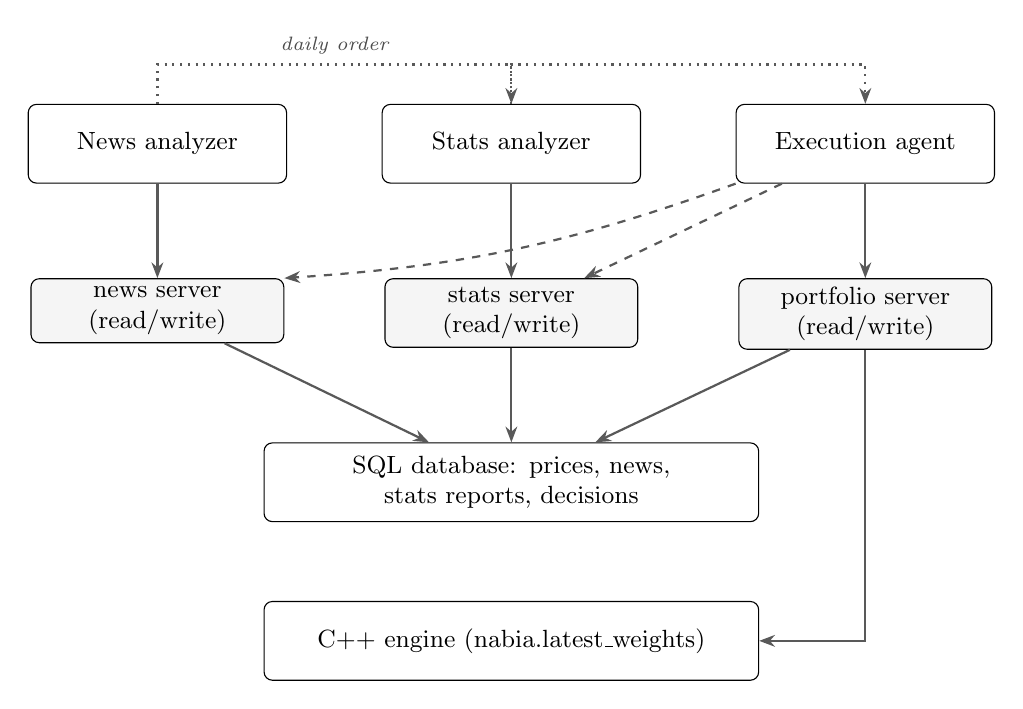
\begin{tikzpicture}[
  box/.style={draw, rounded corners=3pt, align=center, minimum height=10mm, font=\small, fill=white, inner sep=4pt, text width=30mm},
  srv/.style={draw, rounded corners=3pt, align=center, minimum height=8mm, font=\small, fill=gray!8, inner sep=3pt, text width=30mm},
  arrow/.style={-{Stealth[length=2mm]}, thick, gray!70!black},
  lbl/.style={font=\scriptsize\itshape, gray!60!black}]
  \node[box] (news) {News analyzer};
  \node[box, right=12mm of news] (stats) {Stats analyzer};
  \node[box, right=12mm of stats] (exec) {Execution agent};
  \node[srv, below=12mm of news] (sn) {\code{news} server\\(read/write)};
  \node[srv, below=12mm of stats] (ss) {\code{stats} server\\(read/write)};
  \node[srv, below=12mm of exec] (sp) {\code{portfolio} server\\(read/write)};
  \node[box, below=12mm of ss, text width=60mm] (db) {SQL database: prices, news, stats reports, decisions};
  \node[box, below=10mm of db, text width=60mm] (cpp) {C++ engine (\code{nabia.latest\_weights})};
  \draw[arrow] (news) -- (sn);
  \draw[arrow] (stats) -- (ss);
  \draw[arrow] (exec) -- (sp);
  \draw[arrow, dashed] (exec) -- (ss);
  \draw[arrow, dashed] (exec.south west) to[bend left=8] (sn.north east);
  \draw[arrow] (sn) -- (db);
  \draw[arrow] (ss) -- (db);
  \draw[arrow] (sp) -- (db);
  \draw[arrow] (sp.south) |- (cpp.east);
  \draw[arrow, dotted] (news.north) -- ++(0,5mm) -| node[lbl, above, pos=0.25]{daily order} (stats.north);
  \draw[arrow, dotted] (stats.north) -- ++(0,5mm) -| (exec.north);
\end{tikzpicture}
\caption{The three agents, the MCP servers they use, and their order in the daily pipeline. Dashed arrows: read-only access (the servers run with \code{-{}-read-only}).}
\label{fig:agents}
\end{figure}

\paragraph{Pipelines.}
\begin{itemize}
  \item The \emph{daily} pipeline runs news, then stats, then execution, for today.
  \item The \emph{backtest} pipeline runs stats and execution at each decision date
        (\S\ref{sec:backtest-mode}).
\end{itemize}
Every agent run is stored with its turns, tool calls (inputs and outputs, truncated to
2,000 characters), token usage and any error, which gives a complete audit trail.
\begin{codepointers}
  \codeitem{team_run}{running and recording an agent}
  \codeitem{run_daily}{daily pipeline}
  \codeitem{db_tables}{database tables}
\end{codepointers}

\subsection{Configuration}\label{sec:aiconfig}
Agents, servers and pipeline share one \code{AIConfig}, saved as JSON so that the MCP server
processes read the same settings. Unknown keys are rejected. Validation requires at least
two distinct symbols, $0<b_{\min}\le1/n\le b_{\max}\le1$, a known provider, and no
\code{budgets} in \code{portfolio}, because budgets are what the agents decide.
\begin{center}\footnotesize
\input{config.tex}
\end{center}
\begin{codepointers}
  \codeitem{ai_config}{\code{AIConfig}}
\end{codepointers}

\section{MCP servers and tool catalogue}\label{sec:tools}

\subsection{Design}
Each server is a standalone MCP server over stdio
(\code{python -m nabia.ai.servers.<name> -{}-config ... -{}-run ... [-{}-read-only]}). The agents
use them, and so can any MCP client, for example Claude Code. A server is built in three
layers:
\begin{itemize}
  \item A \code{ServerContext} holds the configuration, the run name and the two stores
        (market data and agent data).
  \item Tools are plain Python functions registered with \code{@tool(server)}.
  \item The MCP library derives each tool's \emph{description} from the function's
        docstring and its \emph{input schema} from the type annotations. The catalogue
        below is extracted from the same source, so it is exactly what the model sees.
\end{itemize}

Four rules apply to every tool.
\begin{description}
  \item[Point in time] Analytical tools take \code{as\_of} (\code{YYYY-MM-DD}) and read only
        data dated on or before it. A test rewrites every price after \code{as\_of} and
        checks that every tool's output is unchanged.
  \item[Errors the model can act on] Anticipated failures, such as wrong symbols or
        out-of-range values, raise \code{ValueError} or \code{KeyError}. The decorator turns
        them into MCP \code{ToolError}s carrying the message, so the model sees why a call
        failed and can correct it. Any other exception would reach the model only as a
        generic error.
  \item[Read-only mode] \code{-{}-read-only} omits the tools that write. The execution agent
        cannot store news or overwrite statistics reports.
  \item[Runs] \code{-{}-run <name>} scopes reports and decisions to a backtest run, or to
        \code{live}, so backtests never mix with live decisions.
\end{description}
\snippet{tool_decorator}{Python}{Tool registration}
\snippet{parse_as_of}{Python}{The as-of date}
\begin{codepointers}
  \codeitem{server_context}{\code{ServerContext}}
  \codeitem{server_prices}{prices up to as\_of, universe check}
  \codeitem{clean}{JSON cleaning (NaN to null, rounding)}
  \codeitem{news_server}{news server}
  \codeitem{stats_server}{stats server}
  \codeitem{portfolio_server}{portfolio server}
\end{codepointers}

\subsection{Catalogue}
The rest of this section is generated from the server sources. For each tool it gives the
description shown to the model, whether the tool writes, the source location, and the
parameters with their types and defaults. The input schemas of the structured tools follow
each server. In the news schemas, \code{Topic} is one of:
\begin{itemize}
  \item monetary\_policy, inflation, growth, labor, earnings, fiscal, geopolitics;
  \item energy, metals, agriculture, crypto, rates, credit, fx, regulation, other.
\end{itemize}
\code{AssetClass} is one of equity\_index, bond\_future, commodity and crypto.

\input{tools.tex}

\section{The agent runtime}\label{sec:runtime}

\subsection{Starting an agent}
\code{AgentRuntime.run} starts the agent's MCP servers as subprocesses. They use the same
Python interpreter and module path, with \code{-{}-config} pointing to the saved
configuration and \code{-{}-run} set to the run name. The runtime then:
\begin{itemize}
  \item initializes a client session per server;
  \item lists the tools of every session and rejects name collisions between servers;
  \item adds the hosted tools, if any (web search and fetch on Claude);
  \item runs the loop.
\end{itemize}
Errors raised inside the loop are re-raised only after the sessions close cleanly.
Otherwise the MCP task groups would wrap them in an \code{ExceptionGroup}.
\begin{codepointers}
  \codeitem{runtime_run}{run: servers, tools, loop}
  \codeitem{server_parameters}{server subprocess parameters}
  \codeitem{runtime_client}{client selection by provider}
\end{codepointers}

\subsection{The loop}
The runtime uses a manual tool-use loop, not an SDK tool runner. One agent talks to several
MCP processes at once, mixes their tools with hosted tools, and records every call. Each
turn proceeds as follows.
\begin{enumerate}
  \item \textbf{Request.} One request carries the system prompt, the tools and the
        conversation so far, plus these options:
        \begin{itemize}
          \item \code{max\_tokens}: 16,000;
          \item adaptive thinking;
          \item the agent's effort level;
          \item prompt caching of the stable prefix (tools, system prompt, history);
          \item server-side refusal fallbacks.
        \end{itemize}
  \item \textbf{Streaming.} The reply is \emph{streamed}. Text and thinking deltas go to
        the log as they arrive, so a job's log follows the model live (\S\ref{sec:web}).
  \item \textbf{Stop reasons.}
        \begin{itemize}
          \item \code{refusal} raises an error naming the category.
          \item \code{pause\_turn} (a long hosted-tool turn) resends the conversation so
                the model can resume.
          \item \code{max\_tokens} is an error.
          \item Any other reason that is not \code{tool\_use} ends the run with the final
                text.
        \end{itemize}
  \item \textbf{Tools.} All \code{tool\_use} blocks of the turn run concurrently. Their
        results return \emph{in one user message}. A failing tool, or a crashed server,
        becomes an error result, so the agent can recover.
\end{enumerate}
A run is limited to 40 turns.
\snippet{runtime_loop}{Python}{The agent loop}
\snippet{runtime_create}{Python}{One streamed model turn}
\snippet{live_output}{Python}{Live logging of streamed output}
\snippet{runtime_call_tool}{Python}{Executing one tool call on its MCP server}

\subsection{Providers}
\begin{description}
  \item[Claude] (\code{provider: "anthropic"}) uses \code{claude-opus-5-5} through the
        Anthropic SDK with the options above.
  \item[Local model] (\code{provider: "ollama"}) uses an adapter that exposes the same
        interface (\code{beta.messages.create} and \code{.stream}) and translates to
        Ollama's chat API:
        \begin{itemize}
          \item the system prompt becomes a system message, and tools become function tools;
          \item assistant \code{tool\_use} blocks become \code{tool\_calls}, and
                \code{tool\_result} blocks become \code{tool} messages (errors prefixed
                \code{ERROR:});
          \item streamed NDJSON chunks become text and thinking deltas, and the merged
                reply becomes the final message;
          \item Claude-only options are ignored, and hosted tools are dropped, so local
                news comes from RSS.
        \end{itemize}
        Model options (temperature 0.2, a 32k context) come from the configuration.
\end{description}
\snippet{ollama_stream}{Python}{Ollama streaming as Anthropic-style events}
\snippet{ollama_response}{Python}{Ollama replies translated to content blocks}
\begin{codepointers}
  \codeitem{ollama_messages}{request translation}
  \codeitem{ollama_chat}{HTTP call, streamed or not}
\end{codepointers}

\section{Agent prompts}\label{sec:prompts}

\subsection{Structure and templating}
Every system prompt has the same five parts:
\begin{enumerate}
  \item the agent's role in a cross-asset trend portfolio;
  \item the \emph{as-of rule};
  \item the portfolio universe;
  \item the job;
  \item a numbered workflow that names the tools to use, ending with the expected output.
\end{enumerate}
\code{AgentTeam.\_fill} fills the templates:
\begin{description}
  \item[\code{\{as\_of\}}] the decision date. In live mode it is today.
  \item[\code{\{universe\}}] one line per portfolio symbol, \code{- SYMBOL: name, asset\_class},
        from the asset table.
  \item[\code{\{as\_of\_rule\}}] the rule below, with the date filled in.
  \item[\code{\{news\_days\}}] the news window of the execution agent (7 by default).
  \item[\code{\{research\}}] the news analyzer's research step. With web access (Claude) it
        adds web search and fetch. With a local model it uses the RSS headlines only.
  \item[\code{\{mode\_note\}}] the backtest note for non-live runs, and empty otherwise.
\end{description}
\prompt{as_of_rule}{The as-of rule (in every system prompt)}
\snippet{team_fill}{Python}{Template filling}
\begin{codepointers}
  \codeitem{team_universe}{the universe lines}
\end{codepointers}

\subsection{News analyzer}
The news analyzer runs with effort \code{medium}, the \code{news} server (writable) and, on
Claude, web search and web fetch (each capped at \code{news\_max\_searches} uses). Its user
message is \emph{``Collect and store the market-moving news for \{as\_of\}.''} The prompt
defines the sentiment and relevance rubric (\S\ref{sec:sentiment}) and requires real URLs
and dates.
\prompt{news_system}{News analyzer system prompt (template)}

\subsection{Stats analyzer}
The stats analyzer runs with effort \code{high} and the \code{stats} server (writable). Its
user message is \emph{``Analyze the portfolio assets as of \{as\_of\} and save the stats
report.''} It must:
\begin{itemize}
  \item judge each asset's trend, volatility regime and diversification;
  \item propose a tilt in $[-1,1]$ proportionate to the evidence;
  \item save a schema-validated report (\code{StatsReport}) covering every symbol.
\end{itemize}
\prompt{stats_system}{Stats analyzer system prompt (template)}

\subsection{Execution agent}
The execution agent runs with effort \code{high}, the \code{news} and \code{stats} servers
read-only, and the \code{portfolio} server. Its user message is \emph{``Decide the risk
budgets for \{as\_of\} and compute the target weights.''} The prompt fixes its decision
policy:
\begin{itemize}
  \item start from equal risk;
  \item tilt mainly on the statistical evidence, using news as a secondary input;
  \item respect the bounds;
  \item keep budgets close to the previous decision because trading costs money, and
        explain any large change.
\end{itemize}
\prompt{execution_system}{Execution agent system prompt (template)}
\prompt{backtest_note}{Backtest note, appended for non-live runs (\code{\{mode\_note\}})}
\snippet{team_calls}{Python}{How each agent is called: prompts, user messages, servers, effort}

\section{Statistics computed for the agents}\label{sec:stats}

All statistics use daily close prices up to \code{as\_of}, over
\code{stats\_history\_days} (400) calendar days. Volatilities are annualized with
$\sqrt{252}$, standard deviations are sample standard deviations, and returns are simple
returns.
\begin{description}
  \item[Aligned returns] keep the dates where all assets have a price, then take returns.
        They are used for correlations only. Single-asset statistics use each asset's own
        history.
  \item[Correlation] is the Pearson correlation matrix $\rho$ of the last $w$ aligned
        returns (60 by default, at least 3). The \emph{average correlation} is
        \[
          \bar\rho=\frac{1}{n(n-1)}\sum_{i\ne j}\rho_{ij}.
        \]
  \item[Rolling volatility] is
        $\sigma^{(w)}=\mathrm{sd}\big(r_{T-w+1..T}\big)\sqrt{252}$ for
        $w\in\{20,60,120\}$. The \emph{volatility percentile} is computed from the series
        $v_s$ of rolling 20-day standard deviations over the last 252 dates:
        \[
          \pi=\frac{1}{|v|}\sum_s\mathbf 1[v_s\le v_T].
        \]
        So $\pi=1$ means the highest of the year.
  \item[Past returns] $P_T/P_{T-n}-1$ for $n\in\{21,63,126,252\}$ observations
        (1, 3, 6 and 12 months).
  \item[Moving-average distance] $P_T/\overline P_n-1$, where $\overline P_n$ is the mean
        of the last $n\in\{50,200\}$ prices.
  \item[Volatility-scaled 12-1 momentum]
        \[
          m=\frac{P_{T-21}/P_{T-252}-1}{\mathrm{sd}(r_{T-251..T})\sqrt{252}} .
        \]
        It is the 11-month return ending one month ago, which skips the short-term
        reversal, measured in units of the asset's own annual volatility.
  \item[Drawdowns] over the last 253 prices: $D_t=1-P_t/\max_{s\le t}P_s$. The tools
        report the current value and the maximum.
  \item[Market regime] combines five numbers:
        \begin{itemize}
          \item $\bar\rho$ over 60 and over 252 aligned returns;
          \item the median volatility percentile;
          \item the share of assets above their 200-day average;
          \item the share of assets with a positive 12-month return.
        \end{itemize}
\end{description}
\snippet{trend_signals}{Python}{Trend signals}
\snippet{rolling_volatility}{Python}{Volatilities and their percentile}
\snippet{market_regime}{Python}{Market regime}
\begin{codepointers}
  \codeitem{correlation_matrix}{correlation matrix}
  \codeitem{average_correlation}{average correlation}
\end{codepointers}

\section{From decisions to positions}\label{sec:decisions}

\subsection{Budget normalization within bounds}
The execution agent proposes positive \emph{relative} budgets $\tilde b$. The tool
\code{set\_risk\_budgets} maps them to budgets with $\sum_ib_i=1$ and
$b_{\min}\le b_i\le b_{\max}$:
\begin{enumerate}
  \item Let $F$ be the set of fixed assets, initially empty. Scale the free assets to fill
        the rest: $b_i=\tilde b_i\,(1-\sum_{j\in F}b_j)/\sum_{j\notin F}\tilde b_j$.
  \item Fix every free asset below $b_{\min}$ at $b_{\min}$, and every one above $b_{\max}$
        at $b_{\max}$.
  \item Repeat until nothing is out of bounds. If every asset ends fixed, renormalize the
        fixed values.
\end{enumerate}
This is well defined whenever $nb_{\min}\le1\le nb_{\max}$, which validation guarantees.
Each pass fixes at least one asset, so it ends after at most $n$ passes. The free assets
keep their proposed \emph{ratios}, so the rule changes the agent's intent as little as the
bounds allow.

The tool returns the budgets and how far the bounds moved each one. \code{preview\_budgets}
shows the same result without saving it.
\snippet{project_budgets}{Python}{Budget normalization}
\snippet{set_risk_budgets}{Python}{The decision tool}

\subsection{Target weights}
\code{compute\_target\_weights} loads at least
$\max(3W+30,\,120)$ calendar days of prices up to \code{as\_of}. It runs
\code{nabia.latest\_weights} with the decided budgets, which is the engine of
\S\ref{sec:engine} restricted to the last rebalance. It stores the weights and leverage
with the decision.

Each decision records who made it, as \code{trend\_rule} or as
\code{agent:<model>} (for example \code{agent:ollama:qwen3.8:latest}). Runs on different
models can therefore be compared.
\snippet{compute_weights}{Python}{Budgets to target weights through the C++ engine}

\subsection{The trend rule baseline}
A transparent, model-free policy is the benchmark that agent policies must beat:
\[
  \tilde b_i=\max\!\big(1+s\cdot\mathrm{clip}(m_i,-1,1),\,10^{-6}\big),\qquad s=0.5,
\]
followed by the same bounded normalization. A missing momentum counts as 0. A strong
uptrend ($m_i\ge1$) gets $1.5\times$ the equal budget before normalization, and a strong
downtrend $0.5\times$. Over 2019--2026, on the default universe with monthly decisions, it
reached a Sharpe ratio of 0.96 against 0.92 for equal risk.
\snippet{trend_tilted_budgets}{Python}{The trend rule}
\begin{codepointers}
  \codeitem{trend_rule_decider}{trend rule as a backtest policy}
\end{codepointers}

\subsection{Backtest mode}\label{sec:backtest-mode}
\paragraph{Decision dates.} The trading dates in $[\text{start},\text{end}]$: every one for
\code{D}, or the last of each week (\code{W-FRI}), month (\code{ME}) or quarter (\code{QE}).

\paragraph{Policies.}
\begin{itemize}
  \item \code{trend\_rule};
  \item \code{ollama} (agents on the local model);
  \item \code{claude} (agents on Claude);
  \item \code{agents} (agents on the configured provider).
\end{itemize}

\paragraph{Procedure.}
\begin{enumerate}
  \item At each date $d$, the policy decides budgets as of $d$. A date that already has a
        decision is skipped, so interrupted backtests resume.
  \item The decisions form a budget schedule. Budgets decided at the close of $d$ apply
        from the rebalance at $d$ on.
  \item One continuous backtest runs with the schedule, together with an equal-risk
        baseline over the same period. The run's policy, period and metrics are stored.
\end{enumerate}
The decision frequency is not the trading frequency: trades follow the parameter
\code{rebalance\_frequency}, and each rebalance uses the latest decision.
\snippet{decision_dates}{Python}{Decision dates}
\snippet{evaluate_decisions}{Python}{Decisions to a backtest, against equal risk}
\begin{codepointers}
  \codeitem{run_backtest}{the backtest loop}
  \codeitem{make_decider}{policy to decider}
  \codeitem{agent_decider}{agent policy (stats, then execution)}
\end{codepointers}

\paragraph{Look-ahead control.} The tools cannot see the future. In backtests, news comes
only from the database (no web access), and the prompt asks the model to treat the decision
date as today. One leak cannot be closed by tooling: the language model was trained on data
up to its knowledge cutoff and may recognize market history before it. Agent backtests
inside that window are therefore optimistic. They are fully out of sample only after the
cutoff.

\section{News: collection, sentiment and relevance}\label{sec:sentiment}

\subsection{Collection}\label{sec:news-collection}
The news analyzer runs once a day in live mode.
\begin{enumerate}
  \item It calls \code{query\_news} for the last two days to see what is already stored.
  \item It gathers candidate stories.
        \begin{itemize}
          \item \code{fetch\_news\_feeds} reads ten public feeds: MarketWatch, CNBC (two),
                Financial Times, Investing.com, CoinDesk, OilPrice, the Federal Reserve, the
                ECB and the Bank of England. The list is configurable. The tool parses RSS
                and Atom, keeps items newer than \code{max\_age\_days}, removes URLs already
                stored, and returns the newest first, with HTML stripped from descriptions.
                A broken feed is reported without hiding the others.
          \item On Claude, web search and fetch also fill gaps and confirm stories.
        \end{itemize}
  \item It keeps 8--20 material stories, classifies them, and stores them with
        \code{store\_news\_articles}, keyed by URL (an upsert).
\end{enumerate}
\snippet{fetch_news_feeds}{Python}{RSS and Atom headlines without stored articles}
\begin{codepointers}
  \codeitem{read_feed}{feed parsing}
\end{codepointers}

\subsection{How sentiment and relevance are produced}
\textbf{Sentiment and relevance are judgements made by the language model for each article.
They are not computed by a statistical model or a word list.} The news analyzer reads the
headline and description, and on Claude possibly the article, then fills the
\code{NewsArticle} schema following the rubric in its prompt:
\begin{description}
  \item[Sentiment] $s\in[-1,1]$ is the \emph{expected price impact on the affected assets}:
        $-1$ clearly bearish, $+1$ clearly bullish, $0$ neutral or mixed. It is relative to
        the assets the story moves, not the tone of the text. A hawkish central bank is
        bearish for bonds even when the article reads upbeat.
  \item[Relevance] $r\in[0,1]$ is the importance of the story for a cross-asset
        portfolio: 1 for portfolio-wide shocks, about 0.5 for a story that moves one asset
        class, and lower for minor items.
  \item[Classification] covers the main topic, the affected asset classes, and the
        portfolio symbols directly affected.
\end{description}
The server validates what the model produces before storing it:
\begin{itemize}
  \item the schema bounds $s\in[-1,1]$ and $r\in[0,1]$;
  \item topic and asset classes from fixed lists;
  \item no future dates;
  \item symbols from the universe.
\end{itemize}
Invalid articles are rejected with a reason the model can act on.
\snippet{news_article}{Python}{Article schema}
\snippet{store_news_articles}{Python}{Validation before storage}

\subsection{Aggregation}
\code{news\_summary} takes the articles $A$ published in the $d$ days up to and including
\code{as\_of} and groups them by topic, asset class and symbol. An article that affects
several classes or symbols counts in each of their groups. For each group $g$ it reports:
\begin{itemize}
  \item the count;
  \item the maximum relevance;
  \item the \textbf{relevance-weighted sentiment}
\[
  S_g=\frac{\sum_{i\in g}s_i\,r_i}{\sum_{i\in g}r_i}.
\]
\end{itemize}
When all relevances in a group are zero, the denominator is replaced by 1, so $S_g=0$.
$S_g$ is a convex combination of the sentiments, so $S_g\in[-1,1]$. Weighting by relevance
lets one portfolio-wide story outweigh several minor ones. The summary also lists the ten
most relevant headlines.

The web application's \emph{News} page shows, over the selected filter, article counts per
day and the simple (unweighted) average sentiment per topic.
\snippet{news_summary}{Python}{Relevance-weighted aggregation}
\begin{codepointers}
  \codeitem{query_news}{article queries}
  \codeitem{store_news}{storage (upsert by URL)}
  \codeitem{web_news}{web News aggregates}
\end{codepointers}

\subsection{Use and limitations}
News is a \emph{secondary} input by design. The execution agent tilts mainly on statistics
and uses news to confirm, temper or flag risks the statistics do not show yet. Because the
scores are model judgements:
\begin{itemize}
  \item \textbf{They are not reproducible across models}, and only approximately across
        runs. Decisions record the model that made them.
  \item \textbf{They are uncalibrated.} A sentiment of $0.6$ has no defined relation to a
        return. Using them as quantitative signals would require calibration first, for
        example a regression of next-day returns on $S_g$.
  \item \textbf{Coverage depends on the sources.} RSS headlines and descriptions are short,
        and web access gives fuller context.
\end{itemize}
Possible improvements:
\begin{itemize}
  \item an ensemble of scoring models;
  \item a lexicon or finance-tuned classifier as a reproducible baseline;
  \item a calibration study of $S_g$ against returns.
\end{itemize}

%==============================================================================
\part{Operation}

\section{Web application and job runner}\label{sec:web}

\code{nabia.web} is a FastAPI application with a single-page JavaScript front end
(Chart.js). Start it with
\code{PYTHONPATH=python python -m nabia.web -{}-config ai\_config.json}; it binds to
127.0.0.1 by default.
\begin{center}\small
\begin{tabularx}{\linewidth}{@{}l X@{}}
\toprule
Endpoint & Purpose \\
\midrule
\code{GET /api/overview} & latest live decision, data coverage, recent jobs, model \\
\code{GET /api/news} & articles with filters, counts per day, sentiment by topic \\
\code{GET /api/runs}, \code{/api/runs/\{run\}/decisions} & runs and their decisions \\
\code{GET /api/runs/\{run\}/stats\_report} & a run's stats report as of a date \\
\code{GET /api/agent\_runs}, \code{/api/agent\_runs/\{id\}} & agent transcripts (tool calls, usage) \\
\code{GET /api/backtests/\{run\}} & equity, drawdown, metrics, schedule, weights vs equal risk \\
\code{GET /api/jobs}, \code{/api/jobs/\{id\}} & jobs and their status \\
\code{GET /api/jobs/\{id\}/logs?after=} & job log lines after a given id (tailing) \\
\code{POST /api/jobs} & start a job: \code{download}, \code{news}, \code{daily}, \code{backtest} \\
\bottomrule
\end{tabularx}
\end{center}

\paragraph{Jobs.} Jobs run one at a time, in order, in the server's event loop. SQLite
allows one writer, and agent runs are costly. Their status is stored in the database.
Blocking work runs in worker threads so the server stays responsive:
\begin{itemize}
  \item downloads;
  \item the trend rule;
  \item the final C++ backtest.
\end{itemize}

\paragraph{Live logs.} A logging handler stores every record emitted while a job runs,
under that job's id. The id lives in a \emph{context variable}, which follows the job into
its asyncio tasks and worker threads, so concurrent web requests never leak into a job's
log. The log therefore contains:
\begin{itemize}
  \item the pipeline's steps;
  \item each agent turn and each tool call, with input and output previews;
  \item the model's text and thinking as it streams. Long lines arrive in pieces of about
        400 characters, and slow streams every few seconds.
\end{itemize}
Chatty libraries contribute only warnings and errors. While the job runs, the front end
asks every second for the lines after the last one it has, and shows the model's streamed
text and thinking in their own styles.
\snippet{job_log_handler}{Python}{Per-job log capture}
\snippet{job_run}{Python}{Running a job with its log context}
\begin{codepointers}
  \codeitem{web_app}{application and endpoints}
  \codeitem{job_runner}{job runner}
  \codeitem{job_backtest}{backtest job}
  \codeitem{log_viewer}{front-end log viewer}
\end{codepointers}

\section{Verification}\label{sec:verification}
\begin{description}
  \item[C++] (Catch2): 88 test cases.
        \begin{itemize}
          \item Results against closed forms: inverse volatility for uncorrelated equal
                budgets, Gaussian VaR and ES, SES and Kalman steady states, filter gains at
                the band edges.
          \item Optimizer results against known optima, with constraints.
          \item Accounting identities to $10^{-15}$.
          \item No look-ahead, thread-count independence, and invalid input.
        \end{itemize}
        The suites run in debug, under AddressSanitizer with UndefinedBehaviorSanitizer,
        and the multithreaded code under ThreadSanitizer.
  \item[Python] (pytest): offline by default.
        \begin{itemize}
          \item The analytics, and the three MCP servers in process (including the
                no-look-ahead check).
          \item The agent loop over real stdio MCP servers with a scripted model (parallel
                calls, tool errors, paused turns, refusals).
          \item The Ollama translation and streaming against a mock transport, and live
                log chunking.
          \item RSS parsing, the pipeline, and the web API with job logs.
        \end{itemize}
        Opt-in tests download live market data and run the execution agent end to end on a
        local model.
  \item[This document] Its excerpts, prompts, tool catalogue and configuration table are
        extracted at build time. A listed function that no longer exists stops the build.
\end{description}

\section{Limitations and future work}\label{sec:limitations}
\begin{itemize}
  \item \textbf{Gaussian risk.} VaR and ES are Gaussian; fat tails are not modelled. A
        historical or Cornish--Fisher measure would fit the same interface.
  \item \textbf{Continuous futures} jump at rolls. Back-adjusted series would remove
        spurious returns.
  \item \textbf{Asynchronous closes} (Asia against US) bias same-day correlations downwards.
        Multi-day returns or synchronized prices would reduce the bias.
  \item \textbf{News scores} are uncalibrated model judgements (\S\ref{sec:sentiment}).
  \item \textbf{Agent backtests} before the model's knowledge cutoff are optimistic.
  \item \textbf{Jobs} run sequentially. A queue with a PostgreSQL backend would allow
        concurrent jobs.
\end{itemize}

\end{document}
